\documentclass[a4paper,10pt]{article}

\usepackage{tikz}
\usepackage{fullpage}
\usepackage{amsmath,amsthm,amsfonts,amssymb,amscd}
\usepackage{mathtools}
\usepackage{colortbl}
\usepackage{xcolor}
\usepackage{graphicx}
\usepackage{titlesec}
\usepackage{xepersian}
\usepackage{multirow}
\usepackage{caption}
\usepackage{fancyhdr}
\usepackage{mdframed}


% ---------------------------
%      Color Palette
% ---------------------------
\definecolor{BgDark}{HTML}{141420}
\definecolor{BgCard}{HTML}{1E1E2E}
\definecolor{AccentBlue}{HTML}{7AA2F7}
\definecolor{AccentPurple}{HTML}{BB9AF7}
\definecolor{AccentCyan}{HTML}{7DCFFF}
\definecolor{AccentGold}{HTML}{E0AF68}
\definecolor{TextPrimary}{HTML}{CDD6F4}
\definecolor{TextMuted}{HTML}{6C7086}
\definecolor{RuleLine}{HTML}{313244}

\pagecolor{BgDark}
\color{TextPrimary}


% ---------------------------
%  RTL-safe Info Box
% ---------------------------
\newmdenv[
backgroundcolor=BgCard,
fontcolor=TextPrimary,
linecolor=AccentBlue,
linewidth=1.2pt,
rightline=true,   % RTL: accent border on the RIGHT
leftline=false,
topline=false,
bottomline=false,
innerrightmargin=12pt,
innerleftmargin=12pt,
innertopmargin=10pt,
innerbottommargin=10pt,
skipabove=10pt,
skipbelow=10pt,
]{infobox}
% ---------------------------
%        Font Setup
% ---------------------------
\settextfont{Vazir.ttf}[
    BoldFont = Vazir-Bold.ttf,
    Path = fonts/
]
\setlatintextfont{Vazir.ttf}[
    BoldFont = Vazir-Bold.ttf,
    Path = fonts/
]

% ---------------------------
%     Custom Adjustments
% ---------------------------
\renewcommand{\baselinestretch}{1.2}
\renewcommand{\thesection}{\arabic{section}}

% User-defined commands for homework info (adjust as needed)
\newcommand{\HomeworkNumber}{2}
\newcommand{\HomeworkDeadline}{1404/1/15}
\newcommand{\id}{\texttt{\detokenize{@Amir_hossein83}}}



\begin{document}

% ---------------------------------
%           Title Page
% ---------------------------------
\begin{titlepage}
	
	% Background decorations — right-side rectangle + gold horizontal line
	\begin{tikzpicture}[remember picture, overlay]
		% Right-side vertical rectangle (accent block)
		\fill[BgCard]
		([xshift=-2.2cm]current page.north east) rectangle
		(current page.south east);
		\draw[AccentGold!60, line width=0.8pt]
		([xshift=-2.2cm]current page.north east) --
		([xshift=-2.2cm]current page.south east);
	\end{tikzpicture}
	
	\vspace*{2.2cm}
	
	\begin{center}
		% Logo
		
\includegraphics[scale=1.05]{assets/fum-logo.png}\\[1.0cm]
		
		\textcolor{RuleLine}{\rule{8cm}{0.6pt}}\\[0.6cm]
		
		{\Huge \bfseries \textcolor{TextPrimary}{مبانی و کاربردهای هوش مصنوعی}}\\[0.4cm]
		
		\textcolor{RuleLine}{\rule{8cm}{0.6pt}}\\[0.4cm]
		
		{\large \textcolor{AccentCyan}{دانشگاه فردوسی مشهد}}\\[0.1cm]
		{\normalsize \textcolor{TextMuted}{گروه مهندسی کامپیوتر}}\\[0.2cm]
		{\normalsize \textcolor{AccentGold}{دکتر زارعی}}\\[1.6cm]
		{\normalsize \textcolor{TextMuted}{بهار 1405}}\\[0.2cm]
		
		% Homework number — simple, normal size
		{\normalsize \textcolor{TextMuted}{تمرین شماره}}
		{\large \bfseries \textcolor{AccentBlue}{\HomeworkNumber}}\\[1.4cm]
		
		% Deadline badge — gold border
		\setlength{\fboxrule}{0.8pt}%
		\fcolorbox{AccentGold!60}{BgCard}{%
			\begin{minipage}{7cm}
				\centering\vspace{5pt}
				\textcolor{AccentGold}{\bfseries مهلت تحویل: \HomeworkDeadline}
				\vspace{5pt}
			\end{minipage}
		}\\[0.8cm]
		
		% TA box — gold border
		\fcolorbox{AccentGold!60}{BgCard}{%
			\begin{minipage}{8cm}
				\centering\vspace{5pt}
				\textcolor{TextMuted}{مسئول تمرین:} \quad \textcolor{AccentCyan}{\id}
				\vspace{5pt}
			\end{minipage}
		}
	\end{center}
	
\end{titlepage}
% ---------------------------------
%          Instructions Page
% ---------------------------------
\clearpage

\vspace*{4pt}
\begin{center}
	\colorbox{BgCard}{%
		\begin{minipage}{\dimexpr\linewidth-2\fboxsep\relax}
			\centering
			\vspace{6pt}
			{\bfseries\large \textcolor{AccentGold}{دستورالعمل‌ها}}
			\vspace{6pt}
		\end{minipage}%
	}
\end{center}
\vspace{6pt}

\begin{infobox}
	دانشجویان محترم لطفا به موارد زیر توجه فرمایید:
	\begin{itemize}
		\itemsep0.4em
		\item
		تحویل تمرین‌ها فقط از طریق سامانه آموزش مجازی دانشگاه امکان‌پذیر است.
		\item
		تمرین‌ها باید دست‌نویس، خوانا و با استفاده از خودکار آبی یا مشکی و یا به صورت دیجیتالی با استفاده از قلم نوری نوشته شوند.
		\item
		از تمرین‌های حل‌شده دیگران استفاده نکنید. پیامدهای این کار با دانشجو می‌باشد.
		\item
		نوشتن جواب آخر به تنهایی نمره‌ای نداشته و تمام مراحل حل، مشمول نمره می‌باشد.
		\item
		به دلیل موعد از پیش تعیین‌شده تمرین‌ها و برنامه درسی، امکان تمدید تمرین وجود ندارد. همچنین ارسال تمرین پس از موعد تعیین‌شده نمره‌ای نخواهد داشت.
		\item
		نحوه نام‌گذاری فایل پاسخ باید مطابق جدول~\ref{tab:file_format} و به شکل \lr{\texttt{pdf}} باشد.
	\end{itemize}
	
	\vspace{10pt}
	
	% RTL-safe table: use center environment, manual column colors
	\begin{center}
		\arrayrulecolor{RuleLine}
		\begin{tabular}{|>{\columncolor{BgCard}\centering\arraybackslash}p{3cm}|>{\columncolor{BgDark}\centering\arraybackslash}p{7cm}|}
			\hline
			\textcolor{AccentCyan}{\bfseries\lr{Format}} &
			\texttt{\lr{StudentID-Full\_Name-\#HwNo.pdf}} \\
			\hline
			\textcolor{AccentGold}{\bfseries\lr{Example}} &
			\textcolor{TextMuted}{\texttt{\lr{9876543210-Alan\_Turing-\#01.pdf}}} \\
			\hline
		\end{tabular}
		\captionof{table}{\textcolor{TextMuted}{شیوه نام‌گذاری فایل‌ها}}
		\label{tab:file_format}
	\end{center}
	
\end{infobox}


\vspace{8pt}
\textcolor{AccentCyan}{\rule{\linewidth}{0.8pt}}
% ---------------------------------
%          questions
% ---------------------------------
%%%%%%%%%%%%%%%%%%%%%%%%%%%%%%%%%%%%%%%%%%%%%%%%%%%%%%%%%%%%%%%%%%%%%%%%%%%%%%%%%%%%%%%%%%%%%%
%%%%%%%%%%%%%%%%%%%%%%%%%%%%%%%%%%%%%%%%%%%%%%%%%%%%%%%%%%%%%%%%%%%%%%%%%%%%%%%%%%%%%%%%%%%%%%
\section{\textcolor{AccentGold}{سوال اول}}

درستی یا نادرستی عبارات زیر را مشخص کنید و برای هر مورد حداکثر در دو خط دلیل بیاورید.

\begin{enumerate}
	
	\item
	تابع هیوریستیک $h(n)=0$ برای تمام گره‌ها یک هیوریستیک قابل قبول است.
	
	\item
	اگر یک تابع هیوریستیک یکنواخت (\lr{Consistent}) باشد، آنگاه الزاماً قابل قبول (\lr{Admissible}) نیز هست.
	
	\item
	اگر دو تابع هیوریستیک قابل قبول $h_1$ و $h_2$ داشته باشیم، آنگاه تابع
	\[
	h(n)=\max(h_1(n),h_2(n))
	\]
	همواره یک هیوریستیک قابل قبول خواهد بود.
	
	\item
	در روش \lr{Tree-Search} ممکن است یک حالت چندین بار در درخت جستجو ظاهر شود.
	
	\item
	اگر تابع هیوریستیک دقیقاً برابر هزینه واقعی تا هدف باشد، الگوریتم \lr{A*} فقط گره‌های مسیر بهینه را گسترش می‌دهد.
	
	\item
	هر پاسخ بهینه در مسئله اصلی الزاماً یک پاسخ بهینه در \lr{Relaxed Problem} نیز هست.
	
	\item
	در الگوریتم \lr{Graph-Search} اگر هیوریستیک یکنواخت نباشد ممکن است لازم باشد یک گره چندین بار بازگشایی شود.
	
\end{enumerate}

%%%%%%%%%%%%%%%%%%%%%%%%%%%%%%%%%%%%%%%%%%%%%%%%%%%%%%%%%%%%%%%%%%%%%%%%%%%%%%%%%%%%%%%%%%%%%%

\bigskip
\bigskip
\textcolor{AccentCyan}{\rule{\linewidth}{0.4pt}}
%%%%%%%%%%%%%%%%%%%%%%%%%%%%%%%%%%%%%%%%%%%%%%%%%%%%%%%%%%%%%%%%%%%%%%%%%%%%%%%%%%%%%%%%%%%%%%
%%%%%%%%%%%%%%%%%%%%%%%%%%%%%%%%%%%%%%%%%%%%%%%%%%%%%%%%%%%%%%%%%%%%%%%%%%%%%%%%%%%%%%%%%%%%%%
\section{\textcolor{AccentGold}{سوال دوم}}

برای هر یک از گزاره‌های زیر درستی یا نادرستی آن را مشخص کنید.  
در صورت درست بودن، آن را اثبات کنید و در صورت نادرست بودن، با ارائه یک مثال نقض گزاره را رد نمایید.

\begin{enumerate}
	
	\item
	اگر تابع هیوریستیک در الگوریتم \lr{A*} یک تابع ثابت باشد، آنگاه الگوریتم همواره پاسخ بهینه را پیدا می‌کند.
	
	\item
	هر تابع هیوریستیک قابل قبول (\lr{Admissible}) الزاماً یکنواخت (\lr{Consistent}) نیز هست.
	
	\item
	اگر یک هیوریستیک یکنواخت باشد، مقدار تابع $f(n)=g(n)+h(n)$ در طول هر مسیر در درخت جستجو غیرکاهشی خواهد بود.
	
	\item
	اگر دو هیوریستیک قابل قبول $h_1$ و $h_2$ داشته باشیم، آنگاه تابع
	\[
	h(n)=\min(h_1(n),h_2(n))
	\]
	نیز یک هیوریستیک قابل قبول خواهد بود.
	
	\item
	فضای حالت مسئله اصلی همواره زیرمجموعه‌ای از فضای حالت \lr{Relaxed Problem} است.
	
	\item
	در بدترین حالت، الگوریتم \lr{IDA*} ممکن است یک گره را چندین بار در تکرارهای مختلف گسترش دهد.
	
\end{enumerate}

\bigskip
\textcolor{AccentCyan}{\rule{\linewidth}{0.4pt}}
%%%%%%%%%%%%%%%%%%%%%%%%%%%%%%%%%%%%%%%%%%%%%%%%%%%%%%%%%%%%%%%%%%%%%%%%%%%%%%%%%%%%%%%%%%%%%%



%%%%%%%%%%%%%%%%%%%%%%%%%%%%%%%%%%%%%%%%%%%%%%%%%%%%%%%%%%%%%%%%%%%%%%%%%%%%%%%%%%%%%%%%%%%%%%
\section{\textcolor{AccentGold}{سوال سوم}}
دو اصطلاح \lr{performance measure} و \lr{evaluation function} را تعریف کرده و تفاوت آن را در ارتباط با عامل را مشخص کنید.

\bigskip
\bigskip
\textcolor{AccentCyan}{\rule{\linewidth}{0.4pt}}
%%%%%%%%%%%%%%%%%%%%%%%%%%%%%%%%%%%%%%%%%%%%%%%%%%%%%%%%%%%%%%%%%%%%%%%%%%%%%%%%%%%%%%%%%%%%%%
%%%%%%%%%%%%%%%%%%%%%%%%%%%%%%%%%%%%%%%%%%%%%%%%%%%%%%%%%%%%%%%%%%%%%%%%%%%%%%%%%%%%%%%%%%%%%%
\section{\textcolor{AccentGold}{سوال چهارم}}

دو روش \lr{Tree-Search} و \lr{Graph-Search} را در جستجوی فضای حالت تعریف کرده و تفاوت‌های اصلی آن‌ها را توضیح دهید.

سپس به پرسش‌های زیر پاسخ دهید:

\begin{enumerate}
	
	\item
	در روش \lr{Tree-Search} چه مشکلی ممکن است در هنگام وجود حالت‌های تکراری در فضای حالت به وجود آید؟ با ذکر یک مثال کوتاه توضیح دهید.
	
	\item
	در روش \lr{Graph-Search} چگونه از بروز این مشکل جلوگیری می‌شود؟
	
	\item
	اگر در الگوریتم \lr{A*} از روش \lr{Graph-Search} استفاده شود ولی تابع هیوریستیک یکنواخت (\lr{Consistent}) نباشد، چه مشکلی ممکن است در فرآیند جستجو رخ دهد؟ توضیح دهید.
	
\end{enumerate}


%%%%%%%%%%%%%%%%%%%%%%%%%%%%%%%%%%%%%%%%%%%%%%%%%%%%%%%%%%%%%%%%%%%%%%%%%%%%%%%%%%%%%%%%%%%%%%
%%%%%%%%%%%%%%%%%%%%%%%%%%%%%%%%%%%%%%%%%%%%%%%%%%%%%%%%%%%%%%%%%%%%%%%%%%%%%%%%%%%%%%%%%%%%%%
\bigskip
\textcolor{AccentCyan}{\rule{\linewidth}{0.4pt}}

\section{\textcolor{AccentGold}{سوال پنجم}}

یک عامل در یک محیط شبکه‌ای $4\times4$ حرکت می‌کند. عامل از خانه شروع $S$ به سمت خانه هدف $G$ حرکت می‌کند.

\begin{itemize}
	\item عامل در هر گام می‌تواند به یکی از چهار جهت بالا، پایین، چپ یا راست حرکت کند.
	\item هزینه هر حرکت برابر $1$ است.
	\item ورود به خانه‌های مسدود شده مجاز نیست.
	\item برای تخمین هزینه تا هدف از هیوریستیک فاصله منهتن (\lr{Manhattan Distance}) استفاده می‌شود.
\end{itemize}

نقشه محیط به صورت زیر داده شده است:

\begin{center}
	\begin{tabular}{|c|c|c|c|}
		\hline
		S &  & X &  \\
		\hline
		& X &  &  \\
		\hline
		&  & X &  \\
		\hline
		&  &  & G \\
		\hline
	\end{tabular}
\end{center}

در این جدول، خانه‌های با علامت \lr{X} نشان‌دهنده موانع هستند.

\begin{enumerate}
	
	\item
	مقادیر هیوریستیک فاصله منهتن را برای تمام خانه‌های قابل دسترس تا گره هدف $G$ محاسبه کنید.
	
	\item
	با استفاده از الگوریتم \lr{RBFS} ترتیب گسترش گره‌ها را مشخص کنید.(رسم درخت برای هر مرحله تا قبل از \lr{Backtracking} و نوشتن مقادیر \lr{f-value} و \lr{best-alternative} برای گره ها لازم است.) 
	
	\item
	برای هر گره مقادیر $g(n)$، $h(n)$ و $f(n)$ را بنویسید.
	
	\item
	مسیر نهایی که عامل برای رسیدن از $S$ به $G$ انتخاب می‌کند را مشخص کنید.
	
\end{enumerate}


%%%%%%%%%%%%%%%%%%%%%%%%%%%%%%%%%%%%%%%%%%%%%%%%%%%%%%%%%%%%%%%%%%%%%%%%%%%%%%%%%%%%%%%%%%%%%%
%%%%%%%%%%%%%%%%%%%%%%%%%%%%%%%%%%%%%%%%%%%%%%%%%%%%%%%%%%%%%%%%%%%%%%%%%%%%%%%%%%%%%%%%%%%%%%
%%%%%%%%%%%%%%%%%%%%%%%%%%%%%%%%%%%%%%%%%%%%%%%%%%%%%%%%%%%%%%%%%%%%%%%%%%%%%%%%%%%%%%%%%%%%%%
%%%%%%%%%%%%%%%%%%%%%%%%%%%%%%%%%%%%%%%%%%%%%%%%%%%%%%%%%%%%%%%%%%%%%%%%%%%%%%%%%%%%%%%%%%%%%%
\bigskip
\textcolor{AccentCyan}{\rule{\linewidth}{0.4pt}}
\section{\textcolor{AccentGold}{سوال ششم }}

یک سامانه مسیریاب هوشمند قصد دارد کوتاه‌ترین مسیر را برای یک خودروی امدادی در یک نقشه شهری پیدا کند. فرض کنید هزینه هر یال، زمان سفر بر حسب ثانیه است. دو تابع هیوریستیک زیر پیشنهاد شده‌اند:

\begin{itemize}
	\item $h_1(n)$: زمان لازم برای طی کردن فاصله مستقیم تا هدف با فرض سرعت نور.
	\item $h_2(n)$: زمان لازم برای طی کردن فاصله مستقیم تا هدف با فرض حداکثر سرعت مجاز در بزرگراه‌های شهر ($120$ کیلومتر بر ساعت).
\end{itemize}

با توجه به این سناریو به پرسش‌های زیر پاسخ دهید:

\begin{enumerate}
	\item 
	کدام یک از این دو تابع هیوریستیک، \textbf{دقیق‌تر (Informed)} است؟ با ذکر دلیل توضیح دهید که چرا استفاده از تابع ضعیف‌تر ممکن است باعث گسترش گره‌های بیشتری شود.
	
	\item 
	اگر بدانیم در مسیرهای خاصی، ترافیک سنگین وجود دارد و سرعت میانگین به $20$ کیلومتر بر ساعت کاهش می‌یابد، آیا تابعی مانند $h_3(n) = 2 \times h_2(n)$ همچنان یک هیوریستیک \textbf{قابل قبول (\lr{Admissible})} خواهد بود؟ یک مورد را مثال بزنید که این شرط نقض شود.
	
	\item 
	فرض کنید ده تابع هیوریستیک مختلف ($h_1$ تا $h_{10}$) داریم که همگی قابل قبول هستند اما هر کدام در بخش‌های مختلفی از شهر دقت بالاتری دارند. بهترین روش برای ترکیب این ده تابع به طوری که تابع نهایی هم «قابل قبول» باشد و هم «بیشترین دقت» را داشته باشد چیست؟ فرمول آن را بنویسید.
\end{enumerate}

\begin{center}
	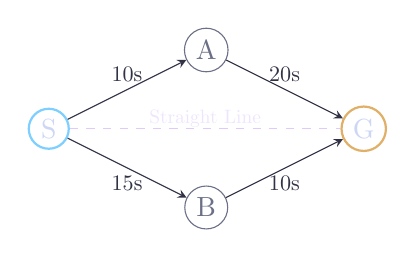
\begin{tikzpicture}
		% Draw a simple graph/map
		\node[circle, draw=AccentCyan, thick, inner sep=2pt] (S) at (0,0) {\textcolor{TextPrimary}{S}};
		\node[circle, draw=TextMuted, inner sep=2pt] (A) at (2,1) {\textcolor{TextMuted}{A}};
		\node[circle, draw=TextMuted, inner sep=2pt] (B) at (2,-1) {\textcolor{TextMuted}{B}};
		\node[circle, draw=AccentGold, thick, inner sep=2pt] (G) at (4,0) {\textcolor{TextPrimary}{G}};
		
		\draw[->, >=stealth, color=RuleLine] (S) -- (A) node[midway, above, scale=0.8] {10s};
		\draw[->, >=stealth, color=RuleLine] (S) -- (B) node[midway, below, scale=0.8] {15s};
		\draw[->, >=stealth, color=RuleLine] (A) -- (G) node[midway, above, scale=0.8] {20s};
		\draw[->, >=stealth, color=RuleLine] (B) -- (G) node[midway, below, scale=0.8] {10s};
		
		\draw[dashed, color=AccentPurple!50] (S) -- (G) node[midway, opacity=0.5, scale=0.7, rotate=0, yshift=5pt] {Straight Line};
	\end{tikzpicture}
	\captionof{figure}{\textcolor{TextMuted}{مدل انتزاعی از گراف شهر برای تحلیل توابع هزینه}}
\end{center}



\bigskip
\textcolor{AccentCyan}{\rule{\linewidth}{0.4pt}}
%%%%%%%%%%%%%%%%%%%%%%%%%%%%%%%%%%%%%%%%%%%%%%%%%%%%%%%%%%%%%%%%%%%%%%%%%%%%%%%%%%%%%%%%%%%%%%
%%%%%%%%%%%%%%%%%%%%%%%%%%%%%%%%%%%%%%%%%%%%%%%%%%%%%%%%%%%%%%%%%%%%%%%%%%%%%%%%%%%%%%%%%%%%%%

%%%%%%%%%%%%%%%%%%%%%%%%%%%%%%%%%%%%%%%%%%%%%%%%%%%%%%%%%%%%%%%%%%%%%%%%%%%%%%%%%%%%%%%%%%%%%%
%%%%%%%%%%%%%%%%%%%%%%%%%%%%%%%%%%%%%%%%%%%%%%%%%%%%%%%%%%%%%%%%%%%%%%%%%%%%%%%%%%%%%%%%%%%%%%
\section{\textcolor{AccentGold}{سوال هفتم }}

یک پهپاد خودران در یک فضای دو بعدی شهری وظیفه دارد بسته‌ای را از نقطه شروع $S$ به نقطه هدف $G$ برساند. در این محیط، علاوه بر ساختمان‌ها (موانع ثابت)، محدودیت مصرف انرژی نیز وجود دارد.

\begin{enumerate}
	\item 
	فرض کنید پهپاد در هر گام می‌تواند به ۸ خانه مجاور (افقی، عمودی و قطری) حرکت کند. هزینه حرکت افقی و عمودی $1$ واحد و هزینه حرکت قطری $\sqrt{2}$ واحد است. یک تابع هیوریستیک «قابل قبول» (\lr{Admissible}) برای این مسئله معرفی کنید که از فاصله اقلیدسی دقیق‌تر باشد.
	
	\item 
	اگر پهپاد دارای محدودیت ارتفاع باشد و بخواهیم هزینه را بر اساس ترکیبی از «مسافت طی شده» و «تغییر ارتفاع» بسنجیم، آیا استفاده از هیوریستیک فاصله منهتن (\lr{Manhattan Distance}) همچنان قابل قبول است؟ پاسخ خود را با ذکر یک مثال نقض یا اثبات کوتاه توضیح دهید.
	
	\item
	مفهوم \textbf{آرام‌سازی مسئله (\lr{Problem Relaxation})} را در نظر بگیرید. اگر شرط «عدم برخورد با ساختمان‌ها» را حذف کنیم، تابع هیوریستیکی که به دست می‌آید چه ویژگی‌هایی خواهد داشت؟ (از نظر بهینه بودن و قدرت تخمین).
\end{enumerate}

\begin{center}
	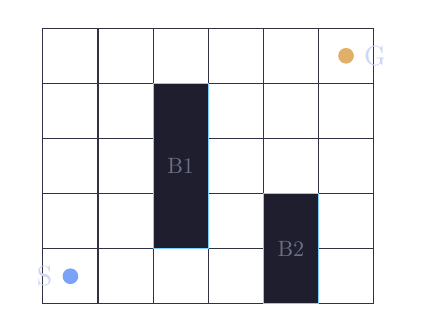
\begin{tikzpicture}[scale=0.7]
		% Grid
		\draw[step=1cm, RuleLine, thin] (0,0) grid (6,5);
		
		% Obstacles
		\fill[BgCard, draw=AccentCyan] (2,1) rectangle (3,4);
		\fill[BgCard, draw=AccentCyan] (4,0) rectangle (5,2);
		
		% Points
		\node[fill=AccentBlue, circle, inner sep=2pt, label=left:\textcolor{TextPrimary}{S}] at (0.5,0.5) {};
		\node[fill=AccentGold, circle, inner sep=2pt, label=right:\textcolor{TextPrimary}{G}] at (5.5,4.5) {};
		
		% Labels
		\node[scale=0.8, text=TextMuted] at (2.5,2.5) {B1};
		\node[scale=0.8, text=TextMuted] at (4.5,1) {B2};
	\end{tikzpicture}
	\captionof{figure}{\textcolor{TextMuted}{نمای شماتیک محیط عملیاتی پهپاد و موانع شهری}}
\end{center}


%%%%%%%%%%%%%%%%%%%%%%%%%%%%%%%%%%%%%%%%%%%%%%%%%%%%%%%%%%%%%%%%%%%%%%%%%%%%%%%%%%%%%%%%%%%%%%


%%%%%%%%%%%%%%%%%%%%%%%%%%%%%%%%%%%%%%%%%%%%%%%%%%%%%%%%%%%%%%%%%%%%%%%%%%%%%%%%%%%%%%%%%%%%%%

% Add more sections as needed...

\end{document}
